% Source: results/uniform_runs.csv (9 unique runs); baseline reused across panels.
\begin{figure}[htbp]
\centering
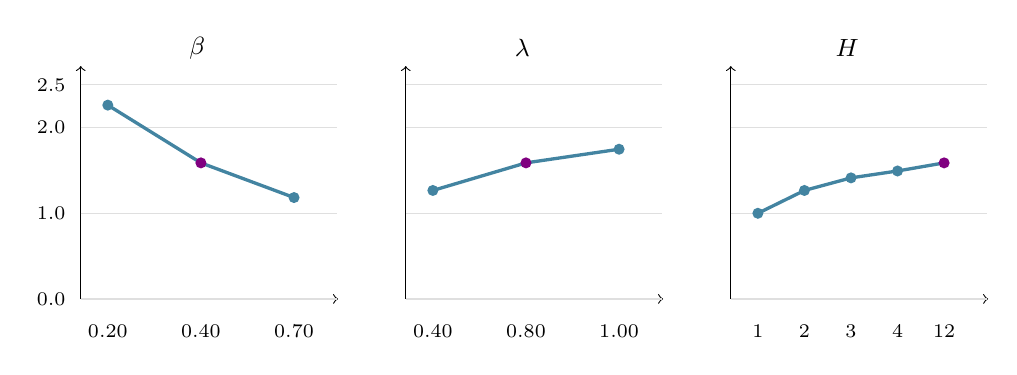
\begin{tikzpicture}[x=.86cm,y=.85cm]
\node[font=\small] at (2.07,4.55) {$\beta$};
\draw[->] (0.35,.80)--(4.15,.80);
\draw[->] (0.35,.80)--(0.35,4.28);
\draw[gray!25] (0.35,0.800)--(4.13,0.800);
\node[font=\scriptsize,anchor=east] at (0.27,0.800) {$0.0$};
\draw[gray!25] (0.35,2.080)--(4.13,2.080);
\node[font=\scriptsize,anchor=east] at (0.27,2.080) {$1.0$};
\draw[gray!25] (0.35,3.360)--(4.13,3.360);
\node[font=\scriptsize,anchor=east] at (0.27,3.360) {$2.0$};
\draw[gray!25] (0.35,4.000)--(4.13,4.000);
\node[font=\scriptsize,anchor=east] at (0.27,4.000) {$2.5$};
\draw[very thick,cyan!60!black] plot coordinates {(0.750,3.696) (2.125,2.833) (3.500,2.315)};
\fill[cyan!60!black] (0.750,3.696) circle (2pt);
\node[font=\scriptsize,anchor=north] at (0.750,.55) {$0.20$};
\fill[violet] (2.125,2.833) circle (2pt);
\node[font=\scriptsize,anchor=north] at (2.125,.55) {$0.40$};
\fill[cyan!60!black] (3.500,2.315) circle (2pt);
\node[font=\scriptsize,anchor=north] at (3.500,.55) {$0.70$};
\node[font=\small] at (6.87,4.55) {$\lambda$};
\draw[->] (5.15,.80)--(8.95,.80);
\draw[->] (5.15,.80)--(5.15,4.28);
\draw[gray!25] (5.15,0.800)--(8.93,0.800);
\draw[gray!25] (5.15,2.080)--(8.93,2.080);
\draw[gray!25] (5.15,3.360)--(8.93,3.360);
\draw[gray!25] (5.15,4.000)--(8.93,4.000);
\draw[very thick,cyan!60!black] plot coordinates {(5.550,2.421) (6.925,2.833) (8.300,3.037)};
\fill[cyan!60!black] (5.550,2.421) circle (2pt);
\node[font=\scriptsize,anchor=north] at (5.550,.55) {$0.40$};
\fill[violet] (6.925,2.833) circle (2pt);
\node[font=\scriptsize,anchor=north] at (6.925,.55) {$0.80$};
\fill[cyan!60!black] (8.300,3.037) circle (2pt);
\node[font=\scriptsize,anchor=north] at (8.300,.55) {$1.00$};
\node[font=\small] at (11.67,4.55) {$H$};
\draw[->] (9.95,.80)--(13.75,.80);
\draw[->] (9.95,.80)--(9.95,4.28);
\draw[gray!25] (9.95,0.800)--(13.73,0.800);
\draw[gray!25] (9.95,2.080)--(13.73,2.080);
\draw[gray!25] (9.95,3.360)--(13.73,3.360);
\draw[gray!25] (9.95,4.000)--(13.73,4.000);
\draw[very thick,cyan!60!black] plot coordinates {(10.350,2.080) (11.037,2.421) (11.725,2.609) (12.412,2.712) (13.100,2.833)};
\fill[cyan!60!black] (10.350,2.080) circle (2pt);
\node[font=\scriptsize,anchor=north] at (10.350,.55) {$1$};
\fill[cyan!60!black] (11.037,2.421) circle (2pt);
\node[font=\scriptsize,anchor=north] at (11.037,.55) {$2$};
\fill[cyan!60!black] (11.725,2.609) circle (2pt);
\node[font=\scriptsize,anchor=north] at (11.725,.55) {$3$};
\fill[cyan!60!black] (12.412,2.712) circle (2pt);
\node[font=\scriptsize,anchor=north] at (12.412,.55) {$4$};
\fill[violet] (13.100,2.833) circle (2pt);
\node[font=\scriptsize,anchor=north] at (13.100,.55) {$12$};
\end{tikzpicture}
\caption{عمق مؤثر بازنمایی $D_{\mathrm{eff}}$ در سیاست یکنواخت با تغییر جداگانه $\beta$، $\lambda$ و $H$. نقطه بنفش در هر سه نمودار همان تنظیم مبنای مشترک است و اجرای تازه‌ای شمرده نمی‌شود.}
\label{fig:ch4-uniform-depth-sensitivity}
\end{figure}
